\documentclass[a4paper]{article}

\usepackage[T2A]{fontenc}
\usepackage[utf8]{inputenc}
\usepackage[russian]{babel}
\usepackage{graphicx}
\usepackage{float}
\usepackage{mathtools}
\usepackage{wrapfig}
\usepackage{amsfonts, amssymb, amsmath, latexsym}
\usepackage{nicefrac}
\usepackage{hhline}
\usepackage{multirow}
\usepackage[colorlinks=true,linkcolor=blue,citecolor=blue]{hyperref}       % hyperlinks
\usepackage{nicefrac}       % compact symbols for 1/2, etc.
\usepackage{nameref}
\usepackage{booktabs}       % professional-quality tables
\usepackage{algorithm}
\usepackage{algpseudocode}
\usepackage{xcolor, colortbl}
\usepackage{etoolbox}
\usepackage{tikz}

% \graphicspath{ {./} }

\usepackage[verbose=true,letterpaper]{geometry}

\newgeometry{
    textheight=25cm,
    textwidth=18cm,
    top=2.5cm,
    headheight=12pt,
    headsep=10pt,
    footskip=1cm,
    marginparwidth=15pt
}

%\usepackage{showframe} 

\usepackage{epigraph}
\usepackage{amsmath,amsfonts,amssymb,amsthm,mathtools, mathrsfs}
\usepackage{amsthm}

\title{Работа 4.7.3 \\ Поляризация}
\author{Шарапов Денис, Б05-005}
\date{}

\usepackage{fancyhdr}
\pagestyle{fancy}
\fancyhf{}
\rhead{Работа 4.7.3}
\lhead{}
\cfoot{\thepage}
\usepackage{subcaption}
\usepackage[font={small}]{caption}

\begin{document}

    \maketitle
    \tableofcontents
    \newpage
    
\section{Аннотация}

\noindent\textbf{Цель работы:} ознакомление с методами получения и анализа поляризованного света. \smallskip
 
\noindent \textbf{В работе используются:} оптическая скамья с осветителем; зелёный светофильтр; два поляроида; чёрное зеркало; полированная эбонитовая пластинка; стопа стеклянных пластинок; слюдяные пластинки разной толщины; пластинки в 1/4 и 1/2 длины волны; пластинка в одну длину волны для зелёного света (пластинка чувствительного оттенка).

\section{Результаты измерений и обработка данных}

\subsection{Определение разрешённых направлений поляроидов}

\begin{figure}[ht!]
    \centering
    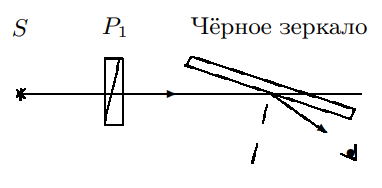
\includegraphics[width = 0.40\textwidth]{image/pic1.png}
    \caption{Определение разрешенных направлений поляроида}
\end{figure}

\noindent Поворачивая поляроид вокруг направления луча, а чёрное зеркало вокруг вертикальной оси, методом последовательных приближений добьемся наименьшей яркости отражённого пятна. Определим разрешённое направление поляроида. По лимбу оно равно

$$ x = 310^{\circ} $$. 

\noindent Поставим вместо чёрного зеркала второй поляроид и определим
его разрешённое направление, скрестив поляроиды. Получаем $$ x = 25^{\circ}.$$
 

\subsection{Определение угла Брюстера для эбонита}

\noindent Поставим на скамью вместо чёрного зеркала (рис. 1) эбонитовую пластину и определим по лимбу угол Брюстера. Получим $$ \theta =(54 \pm 4) ^\circ,$$ $$n = \tan{\theta} = 1,38 \pm 0,08.$$ 

\subsection{Исследование стопы}


\begin{figure}[ht!]
    \centering
    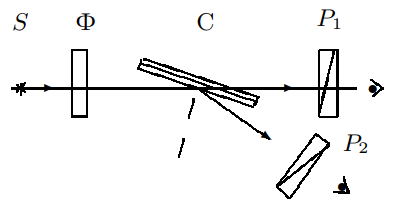
\includegraphics[width = 0.35\textwidth]{image/pic2.png}
    \caption{Исследование стопы}
\end{figure}

\noindent Исследуем характер поляризации света в преломлённом и отражённом от стопы лучах. Для этого поставим вместо эбонитового зеркала (рис. 1) стопу стеклянных пластинок под углом Брюстера. Осветим стопу неполяризованным светом и, рассматривая через поляроиды (рис. 2) отражённый от стопы и преломлённый лучи, определим в них ориентацию вектора $ \mathbf{E} $. \medskip

\noindent Получим, что он отклоняется от направления распространения света на угол $$ \varphi = \pi/2. $$

\subsection{Определение главных плоскостей двоякопреломляющих пластин}

\begin{figure}[ht!]
    \centering
    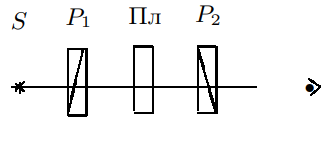
\includegraphics[width = 0.35\textwidth]{image/pic3.png}
    \caption{Определение главных направлений в пластинках}
\end{figure}

\noindent Определим главные направления двоякопреломляющих пластин. Для этого поставим кристаллическую пластинку между скрещенными поляроидами (рис. 3). Вращая пластинку вокруг направления луча и наблюдая за интенсивностью света, проходящего сквозь второй поляроид, определим, при каком условии главные направления пластинки совпадают с разрешёнными направлениями поляроидов. 

\subsection{Выделение пластин в 1/4 и 1/2 длины волны}

\noindent Для выделения пластин $ \lambda/2, \; \lambda/4 $ добавим к схеме, изображённой на рис. 3, зелёный фильтр и установим разрешённое направление первого поляроида горизонтально, а главные направления исследуемой пластинки --- под углом $ 45^\circ $ к горизонтали. C помощью второго поляроида установим, какую поляризацию имеет свет, прошедший пластинку: круговую или линейную с переходом
в другой квадрант. \medskip

\noindent В случае круговой получаем пластинку длиной $ \lambda/4 $, а в случае линейной --- $ \lambda/2 $.

\subsection{Определение направления большей и меньшей скорости в пластинки в 1/4 длины волны}

\begin{figure}[ht!]
    \centering
    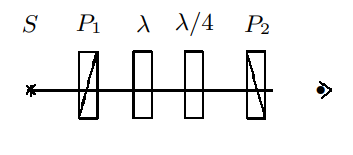
\includegraphics[width = 0.35\textwidth]{image/pic4.png}
    \caption{Определение направлений большей и меньшей скорости}
\end{figure}

\noindent Определим "<быструю"> и "<медленную"> оси в пластинке $ \lambda/4 $. Для этого поставим между скрещенными поляроидами пластинку чувствительного оттенка, имеющую вид стрелки, и убедимся, что эта пластинка не меняет поляризацию зелёного света. Уберем зелёный фильтр и убедимся, что стрелка имеет пурпурный цвет. Это объясняется тем, что зелёная компонента линейно поляризованного света при прохождении пластинки не меняет поляризации и задерживается вторым поляроидом. \medskip

\noindent Добавим к схеме пластинку $ \lambda/4 $ (рис. 4), главные направления которой совпадают с главными направлениями пластины $\lambda$ и ориентированы под углом $ 45^\circ $ к разрешённым направлениям скрещенных поляроидов. При повороте рейтера со стрелкой на $ 180^\circ $ вокруг вертикальной оси цвет стрелки меняется от зелёно-голубого до оранжево-жёлтого. В первом случае наблюдаем <<быструю">> ось, а во втором --- <<медленную>>.

\subsection{Интерференция поляризованных лучей}

Исследуем интерференцию поляризованных лучей. Для этого расположим между скрещенными поляроидами мозаичную слюдяную пластинку. Она собрана из 4-х узких полосок слюды, лежащих по сторонам квадрата (две полоски "<толщиной"> $ \lambda/4 $ и по одной --- $ \lambda/2 $ и $ 3\lambda/4 $). В центральном квадратике слюды нет. Главные направления всех пластинок ориентированы параллельно сторонам квадрата. Вращая пластинку, пронаблюдаем за изменениями в отдельном квадратике. Заметим, что изменяется интенсивность. Не трогая пластинки, повращаем второй поляроид. Отличие в том, что теперь изменяется цвет.

\subsection{Определение направления вращения светового вектора в эллиптически поляризованной волне}


\begin{figure}[!ht]
    \centering

\tikzset{every picture/.style={line width=0.75pt}} %set default line width to 0.75pt        

\begin{tikzpicture}[x=0.75pt,y=0.75pt,yscale=-1,xscale=1]
%uncomment if require: \path (0,300); %set diagram left start at 0, and has height of 300

%Straight Lines [id:da3237926564538498] 
\draw    (290,148.02) -- (290,21.02) ;
\draw [shift={(290,19.02)}, rotate = 90] [color={rgb, 255:red, 0; green, 0; blue, 0 }  ][line width=0.75]    (10.93,-3.29) .. controls (6.95,-1.4) and (3.31,-0.3) .. (0,0) .. controls (3.31,0.3) and (6.95,1.4) .. (10.93,3.29)   ;
%Straight Lines [id:da6865908031163899] 
\draw    (181.28,88.02) -- (423.28,88.02) ;
\draw [shift={(425.28,88.02)}, rotate = 180] [color={rgb, 255:red, 0; green, 0; blue, 0 }  ][line width=0.75]    (10.93,-3.29) .. controls (6.95,-1.4) and (3.31,-0.3) .. (0,0) .. controls (3.31,0.3) and (6.95,1.4) .. (10.93,3.29)   ;
%Shape: Ellipse [id:dp9216742680389198] 
\draw   (236.36,86.52) .. controls (236.36,69.59) and (260.38,55.87) .. (290,55.87) .. controls (319.62,55.87) and (343.64,69.59) .. (343.64,86.52) .. controls (343.64,103.45) and (319.62,117.17) .. (290,117.17) .. controls (260.38,117.17) and (236.36,103.45) .. (236.36,86.52) -- cycle ;
%Curve Lines [id:da06414894036423968] 
\draw    (324.28,63.02) .. controls (303.4,55.19) and (309.77,57.96) .. (305.19,57.49) ;
\draw [shift={(302.28,57.02)}, rotate = 11.31] [fill={rgb, 255:red, 0; green, 0; blue, 0 }  ][line width=0.08]  [draw opacity=0] (10.72,-5.15) -- (0,0) -- (10.72,5.15) -- (7.12,0) -- cycle    ;
%Curve Lines [id:da5363019778615428] 
\draw    (264.28,112.02) .. controls (258.67,112.95) and (256.56,109.52) .. (267.75,114.79) ;
\draw [shift={(270.28,116.02)}, rotate = 206.57] [fill={rgb, 255:red, 0; green, 0; blue, 0 }  ][line width=0.08]  [draw opacity=0] (10.72,-5.15) -- (0,0) -- (10.72,5.15) -- (7.12,0) -- cycle    ;

% Text Node
\draw (421,93) node [anchor=north west][inner sep=0.75pt]   [align=left] {$\displaystyle x$};
% Text Node
\draw (271,12) node [anchor=north west][inner sep=0.75pt]   [align=left] {$\displaystyle y$};

\end{tikzpicture}

\caption{Направление вращения электрического вектора в эллиптически поляризованной волне}
\end{figure}

\begin{figure}[!ht]
    \centering    



    \tikzset{every picture/.style={line width=0.75pt}} %set default line width to 0.75pt        

    \begin{tikzpicture}[x=0.75pt,y=0.75pt,yscale=-1,xscale=1]
    %uncomment if require: \path (0,168); %set diagram left start at 0, and has height of 168
    
    %Straight Lines [id:da7951174719320984] 
    \draw    (285,157.02) -- (285,25.07) ;
    \draw [shift={(285,23.07)}, rotate = 90] [color={rgb, 255:red, 0; green, 0; blue, 0 }  ][line width=0.75]    (10.93,-3.29) .. controls (6.95,-1.4) and (3.31,-0.3) .. (0,0) .. controls (3.31,0.3) and (6.95,1.4) .. (10.93,3.29)   ;
    %Straight Lines [id:da8639838223731073] 
    \draw    (176.28,97.02) -- (468.28,97.02) ;
    \draw [shift={(470.28,97.02)}, rotate = 180] [color={rgb, 255:red, 0; green, 0; blue, 0 }  ][line width=0.75]    (10.93,-3.29) .. controls (6.95,-1.4) and (3.31,-0.3) .. (0,0) .. controls (3.31,0.3) and (6.95,1.4) .. (10.93,3.29)   ;
    %Curve Lines [id:da27525720434755185] 
    \draw    (285,96.52) .. controls (317.28,-62.56) and (332.28,254.44) .. (364.28,97.44) ;
    %Curve Lines [id:da32241407741183425] 
    \draw    (205.72,95.6) .. controls (238,-63.48) and (253,253.52) .. (285,96.52) ;
    %Curve Lines [id:da058541509146419424] 
    \draw    (364.28,97.44) .. controls (396.56,-61.64) and (411.56,255.36) .. (443.56,98.36) ;
    %Shape: Free Drawing [id:dp8186214727985697] 
    \draw  [draw opacity=0][line width=3] [line join = round][line cap = round] (440.28,94.44) .. controls (449.44,108.17) and (464.28,126.52) .. (464.28,143.44) ;
    %Curve Lines [id:da3672506391150274] 
    \draw    (188,95.52) .. controls (220.28,-63.56) and (235.28,253.44) .. (267.28,96.44) ;
    %Curve Lines [id:da9046791222043027] 
    \draw    (267.28,96.44) .. controls (299.56,-62.64) and (314.56,254.36) .. (346.56,97.36) ;
    %Curve Lines [id:da8918132498586309] 
    \draw    (346.56,97.36) .. controls (378.84,-61.73) and (393.84,255.27) .. (425.84,98.27) ;
    %Straight Lines [id:da027791567819379415] 
    \draw    (348.28,47.07) -- (357.28,60.07) ;
    %Straight Lines [id:da3075562237317997] 
    \draw    (393.28,64.07) -- (403.28,52.07) ;
    
    % Text Node
    \draw (462,103) node [anchor=north west][inner sep=0.75pt]   [align=left] {$\displaystyle t$};
    % Text Node
    \draw (252,12) node [anchor=north west][inner sep=0.75pt]   [align=left] {$\displaystyle f( t)$};
    % Text Node
    \draw (329,27) node [anchor=north west][inner sep=0.75pt]   [align=left] {$\displaystyle x( t)$};
    % Text Node
    \draw (397,30) node [anchor=north west][inner sep=0.75pt]   [align=left] {$\displaystyle y( t)$};
    
    
    \end{tikzpicture}
    
\caption{Графики двух вышедших из пластинки синусоид со сдвигом фаз в четверть периода}
\end{figure}

Для определения направления вращения светового вектора в эллипсе
установим между поляроидами дополнительную пластинку $\lambda/4$ с известными направлениями <<быстрой>> и <<медленной>> осей, ориентированными по осям эллипса поляризации анализируемого света.
В этом случае вектор $\mathbf{E}$ на выходе будет таким, как если бы свет прошёл две пластинки $\lambda/4$: свет на выходе из второй пластинки будет линейно поляризован. Если пластинки поодиночке дают эллипсы, вращающиеся в разные стороны, то поставленные друг за другом, они скомпенсируют разность фаз, и вектор $\mathbf{E}$ на выходе останется в первом и третьем квадрантах. Если же световой вектор перешёл в смежные квадранты, значит, эллипсы вращаются в одну сторону.

\section{Вывод}

Поляризованный свет обладает большим числом свойств, которые можно
применять для исследования оптических характеристик различных приборов и веществ.

\end{document}
